\chapter{Introduction}
	\section{Principe des lasers}
	\begin{wrapfigure}[8]{l}{6cm}
	\vspace{-5mm}
	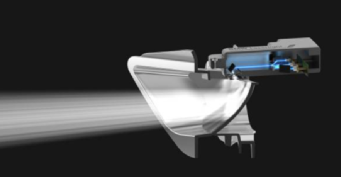
\includegraphics[scale=0.5]{ch1/image1.png}
	\captionof{figure}{ }
	\end{wrapfigure}
	Avant d'en venir au principe des lasers, demandons-nous ce qu'est un laser, et qu'est ce qu'une "lumière
	laser" ? Le "phare laser" utilisé dans les Audi est-il une émission laser ? En réalité non car la lumière 
	est non monochromatique et non cohérente : l'appellation vient du fait que ce phare utilise un laser bleu 
	pour pomper, la conversion optique/électrique étant importante.\\
	
	Un \textbf{laser} est \textit{un oscillateur optique faisant recours à l'émission stimulée}. Afin de clarifier 
	la notion d'oscillateur, voici un exemple d'oscillateur acoustique avec l'effet Larsen. L'effet Larsen 
	est une oscillation acoustique auto-entretenue dans une boucle constitué d'un microphone et d'un haut 
	parleur. Si le microphone est trop prêt du haut-parleur, une partie va être capté et amplifiée (seulement les
	fréquence de 20 à 20 kHz) via la rétroaction. 

	\begin{center}
			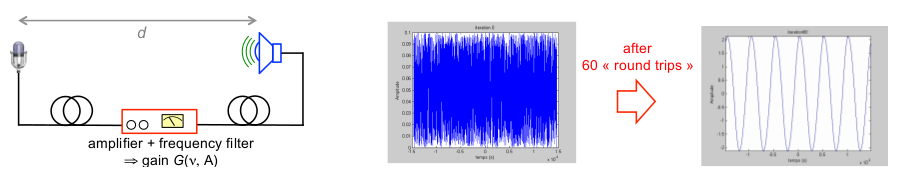
\includegraphics[scale=0.5]{ch1/image2.png}
	\captionof{figure}{ }
		\end{center}	
	
	En modélisant numériquement le système et en lui fournissant un bruit en entrée, après une soixantaine de 
	passage dans la boucle on observe un signal sinusoïdal : c'est le sens strident entendu. Ceci n'est possible 
	que si il y a amplification, le "bruit" ayant une faible amplitude.\\
	
	Essayons de modéliser une telle boucle. Si le gain sur une boucle est supérieur aux pertes, nous aurons bien 
	une amplification même si les perturbations sont petites. Cependant,le gain ne peut pas augmenter de façon
	infinie. On modélise cette \textbf{saturation}
	\begin{equation}
	G = \dfrac{G_0}{1+\dfrac{A}{A_S}}
	\end{equation}
	où $A_0$ est le gain à petit signaux. Limiter le gain n'est pas suffisant : il faut que le système se 
	stabilise vers un état stationnaire. Imaginons qu'à un moment, le microphone capte une onde accoustique 
	monofréquence :
	\begin{equation}
	\delta P_n = A\cos(2\pi\nu t)
	\end{equation}
	Après un premier tour dans la boucle, on obtient
	\begin{equation}
	\delta P_{n+1} = A\cos(2\pi\nu t+\delta\varphi)G(\nu)\alpha(\nu,d)
	\end{equation}
	où l'on a pris un certain déphasage qui peut s’exprimer 
	\begin{equation}
	\Delta\varphi = \frac{2\pi d}{\lambda}+\phi_{elec}
	\end{equation}
	où $\phi_{elec}$ est le déphasage induit par l'amplificateur et où $\lambda_0\nu_0=c$. Ce déphasage est 
	multiplié par un gain $G$ mais nous avons aussi une certaine atténuation par propagation (seule une 
	petite partie est captée par le microphone.\\
		
	Nous serons en condition stationnaire à la fréquence $\nu_0$ lorsque
	\begin{equation}
	\delta P_n=\delta P_{n+1}
	\end{equation}
	Ceci n'est possible que si les gains sont équivalents au pertes et si le déphasage est un multiple de $2\pi$.
	\begin{equation}
	\left\{\begin{array}{lll}
	\text{Amplitude } &\ : G(\nu_0)\alpha(\nu_0,d) &= 1\\
	\text{Phase } &\ : \Delta\varphi &= m2\pi\\	
	&\ : (m-\phi_{elec}/2\pi)\lambda_0 &= d
	\end{array}\right.
	\end{equation}
	Un laser en régime sera dans une telle situation. Mais pour avoir un laser, il faut un gain et une 
	rétroaction positive. Pour avoir du \textit{feedback} en acoustique, on utilise un microphone. En 
	optique, nous l'obtiendrons à l'aide de miroirs formant une cavité optique (\textit{résonator}). Deux 
	d'entre eux sont largement répandus : la cavité linéaire de Fabry-Perot et la cavité circulaire
	
	
	\begin{center}
	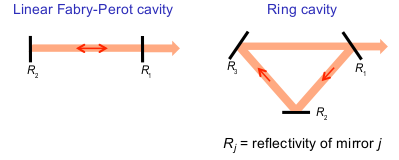
\includegraphics[scale=0.75]{ch1/image3.png}
	\captionof{figure}{ }
	\end{center}	
	Avec un Fabry-Perot, on peut placer un milieu à gain pour avoir un effet de rétroaction. De façon 
	générale, Fabry-Perot désigne un résonateur où la lumière fait des allers-retours.
	
	La \textit{condition de résonance} s'énonce
	\begin{equation}
	kL = \frac{2\pi}{\lambda}L = m2\pi\qquad\Leftrightarrow\qquad \nu = l\frac{c}{L}
	\end{equation}
	où $L$ est la longueur de la cavité\footnote{Prendre le double de la longueur entre deux miroirs pour
	un Fabry-Perot.} Dans un laser, seulement quelques fréquences optiques peuvent en sortir : ce sont celles 
	qui satisfont cette condition. Ils portent le nom de \textit{modes}. Ainsi, ette condition établi la 
	fréquence des modes longitudinaux dans le résonateur optique. Notons que pour être dans le visible, les 
	ordres doivent être très élevés.
	
	\newpage	
	\begin{wrapfigure}[16]{r}{6.5cm}
%	\vspace{-5mm}
	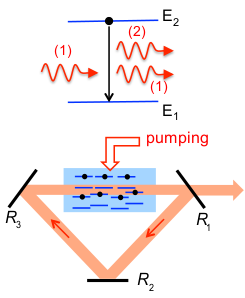
\includegraphics[scale=0.65]{ch1/image4.png}
	\captionof{figure}{ }
	\end{wrapfigure}	
	Une cavité n'est pas suffisante pour avoir un laiser, il faut aussi un gain optique. En effet, 'Laser' est
	l’acronyme de \textbf{l}ight \textbf{a}mplification by \textbf{s}timulated \textbf{e}mission \textbf{r}adiation.
	Or, il manque quelque chose dans cet acronyme ; l’émission stimulée, postulée par Einstein. Si les 
	atomes peuvent capturer de la lumière, ils peuvent également en émettre. Dès lors, si l'énergie d'un photon 
	est proche de la différence entre deux niveaux d'énergie $(E_1$ et $E_2$), il est émis un photo indistinguable 
	du photon incident (même fréquence, même direction, même état de polarisation et phase identique).\\
	
	En pratique, on utilise un milieu à gain : un paquet d'atomes excité dans l'état $E_2$ grâce à un mécanisme 
	de pompage.\\
	
	\begin{wrapfigure}[11]{l}{6.5cm}
	\vspace{-5mm}
	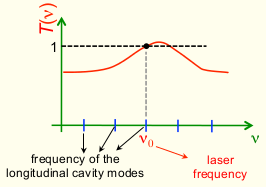
\includegraphics[scale=0.65]{ch1/image5.png}
	\captionof{figure}{ }
	\end{wrapfigure}
	Considérons le produit pertes-gain
	\begin{equation}
	T(\nu) = R_1R_2R_3\exp(-\alpha_iL)\exp(\mathcal{G}d) =1
	\end{equation}
	où $d$ est la longueur du milieu à gain, $\alpha_i$ les pertes internes (diffusion d'un laser dans l'eau,\dots),
	$R_i$ les coefficients de réflexivité et $\mathcal{G}$ le gain.
	
	Si $T(\nu) > 1$, il y a plus de gain que de perte : amplification du gain dans la cavité. L'intensité va 
	augmenter mais le gain diminuer (saturation) de sorte à évoluer vers le cas stationnaire.\\
	
	Cependant, il faut que l'effet laser démarre : ceci sera possible grâce à l'émission spontanée. Ce principe 
	est très général mais est applicable à tous laser. La diversité de lasers est donc très importante :
	\begin{description}
	\item[Taille du laser] : quelques micromètres à des centaines de kilomètres
	\item[Milieu à gain] : gaz, ions, semi-conducteurs, \dots
	\item[Pompage] : pompage laser (on  utilise un laser pou exciter les atomes du milieu à gain le temps qu'un 
	photon arrive pour provoquer une émission), électrique (énergie des électrons), \dots
	\end{description}


	\section{Caractéristiques des sources lasers}
	Une source laser n'est certainement pas équivalente à une source thermique. On retrouve pour les sources 
	laser :
	\begin{itemize}
	\item[$\bullet$] Quasi-monochromatique\footnote{Pas nécessairement monochromatique, mais dépasse le cadre 
	du cours.}
	\item[$\bullet$] Grande directivité
	\end{itemize}
	Ces deux caractéristiques se cachent sous le nom de \textit{cohérence spatiale} et \textit{temporelle}. 
	
	\subsection{Cohérence temporelle}
	Soit $\cos(\omega t)$. Si après certains temps on ne peut plus prédire la phase de l'onde, la lumière n'est 
	plus \textit{temporellement cohérente}. Si on observe des sauts de phase, elle sera dite \textit{partiellement 
	cohérente}. La cohérence temporelle est donc l'intervalle temporel dans lequel on peut prédire la phase. \\
	
	\begin{wrapfigure}[11]{l}{6.5cm}
	\vspace{-5mm}
	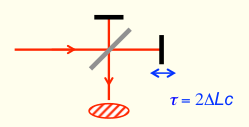
\includegraphics[scale=0.65]{ch1/image6.png}
	\captionof{figure}{ }
	\end{wrapfigure}
	Si les deux bras d'un interféromètre n'ont pas la même longueur, un délai temporel va apparaître et il est 
	possible d'observer des franges d'interférences. Mais plus on éloigne le miroir, plus cette visibilité 
	diminue jusqu'à ce que l'on observe plus rien\footnote{Ceci est du à un défilement trop rapide des franges
	 d'interférences.}. Ceci est la longueur de cohérence $L_C$, liée par la relation
	\begin{equation}
	\tau_c = L_Cc
	\end{equation}
	
	Il existe un lien entre $\tau_c$ et la largeur spectrale de la source :
	\begin{equation}
	\delta\nu \approx \frac{1}{\tau_c}
	\end{equation}
	Pour le soleil $\Delta\nu =4*10^{14}\ Hz \to \tau_c = 2.5\ fs, L_c=0.7\ \mu m$. Pour l'émission d'une raie
	Néon à 633 nm, on trouve une longueur de cohérence de 2 cm. Ces deux longueurs sont trop court pour des 
	applications comme de l'interférométrie. Par contre, à l'aide d'un laser qui possède une largeur 
	spectrale de $\Delta \nu  = 500\ Hz$, on trouve $L_c=600\ km$ ce qui est beaucoup plus intéressant!
	
	
	\subsection{Cohérence spatiale}
	Nous regardons cette fois-ci dans l'espace. Connaissant le champ à un endroit, sommes-nous capable de 
	le prédire à un autre ? Considérons une source composée de points sources indépendants les uns des autres 
	et plaçons un plan $\Sigma$ possédant deux trous à une distance $D$ de la source. Plaçons ensuite un écran 
	$\Sigma_0$ comme le suggère l'image ci-dessous

	\begin{center}
	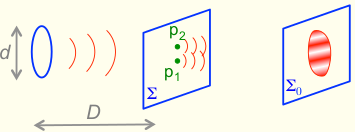
\includegraphics[scale=0.75]{ch1/image7.png}
	\captionof{figure}{ }
	\end{center}
\newpage	
	Si les franges sur $\Sigma_0$ sont fixes, c'est que la phase est constante : si ce n'est pas le cas, les 
	franges défilerons et les points $p_1$ et $p_2$ seront dit incohérent l'un par rapport à l'autre. Il est 
	possible démontrer que les franges sont visibles sur $\Sigma_0$ si
	\begin{equation}
	\nu = 2	\left|\dfrac{J_1\left(\dfrac{\pi\Delta x d}{\overline{\lambda}D}\right)}{\left(\dfrac{\pi\Delta x d}{\overline{\lambda}D}\right)}\right|
	\end{equation}
	où $J_1$ est la fonction de Bessel, $\overline{p_1p_2}= \Delta x$ et $\overline{\lambda}$ est la longueur d'onde moyenne.\\
	
	Si à $D=1m$ et $|p_1-p_2|< 30\ \mu m$ on verra les franges de Youg : ce n'est pas très cohérent. Par contre 
	en grossissant la sortie d'un laser on peut avoir deux mètre d'écart pour $\Delta x$ ce qui est bien mieux.
	
	
	\subsubsection{Application}
	La fin du chapitre illustre les différentes applications que l'on peut trouver avec des lasers.
	
	
	
	
	
	
	
	
	
	
	
	
	
	
	
	
	
	
	
	
	
	
	
	